\documentclass[openany]{article}
\usepackage[english]{babel}
\usepackage{commands}
\usepackage{xcolor}
\usepackage{caption}
\usepackage{graphics}
\usepackage{minted}
\usepackage{caption}
\usepackage{subcaption}
\usepackage{graphicx}
\usepackage{multicol,lipsum}
\usepackage{appendix}
\usepackage{lipsum}
\usepackage{mwe}
\usepackage{amsmath}


\pagestyle{fancy}
\fancyhf{}
\lhead{}
\rhead{\leftmark}
\cfoot{\thepage}

\usepackage{biblatex} %Imports biblatex package
\addbibresource{refs.bib}

\begin{document}

\counterwithout{equation}{section}

\thispagestyle{empty}    

\begin{titlepage}
\begin{figure}[th]
\begin{flushleft}
    
\includegraphics[width=7cm]{ugr.png}
\end{flushleft}
\end{figure}
 \vspace{1cm}

{\flushleft \LARGE \bfseries MASTER'S THESIS\par}\vspace{2cm}

% Thesis title
{\flushright \LARGE \bfseries Mixed Monte Carlo - Convolutional Neural Network model for stereotactic radiosurgery with a dynamic micro-
multileaf collimator  \par}\vspace{2cm}

{\flushleft \LARGE \bfseries Armando Delgado Fumero \par}\vspace{1.5cm}

{\flushleft \bfseries Master’s Degree in Physics and Mathematics \par}\vspace{0.cm}

{\flushleft \small \bfseries Academic Year 2021/2022\par}
{\flushleft \small \bfseries Supervisors:
\begin{itemize}
    \item Luis Díaz Angulo (UGR)
    \item Wilfredo González (UMA)
\end{itemize}}\vspace{2cm}



\end{titlepage}

\clearpage\thispagestyle{empty}\null\newpage %blank page
	
\pagenumbering{arabic}


\newpage
\thispagestyle{plain}
{
\hypersetup{hidelinks}
\tableofcontents
}

\newpage 

\listoffigures
\listoftables

\newpage 

\thispagestyle{empty}


\thispagestyle{plain}

\section{Abstract}

Based on the work of González (2015) \cite{Gonzalez2015}, our goal is to develop a mixed Monte Carlo - Deep Learning based solution that allow us to predict the fluence outcome of a 6 MV Elekta Precise linac. This project goes through two main steps, first, we use Fippel et al (2003) \cite{Fippel} VSM (Virtual Source Model) to get a first approximation to the data, obtaining an equation composed of a Pearson VII distribution modified by another custom equation that defines a depression on the center of each profile. Monte Carlo step of this VSM is used to obtain 6, 5 coefficients that define the central depression present on the profile and a sixth one that defines how abrupt the fluence zone ends. After obtaining this function which approximates the fluence results, we train and test a 1 Dimensional Convolutional Neural Network, improving the results of the analytic function on a 20\% basis.

    \vspace{2cm}
    




\pagenumbering{arabic}

\newpage

\section{Introduction} \label{sec: introduction}

\subsection{Linac}


A linear acelerator (linac) is an artifact that uses microwave technology to initially accelerate electrons on a wave guide. These accelerated electrons hit a metal target, which produces x-rays. These photons product of the collision are directed towards the machine exit, shaped as the physician requires. These machines are used mainly on cancer treatments, delivering the radiation to the tumor.

\begin{figure}[!h]
    \centering
    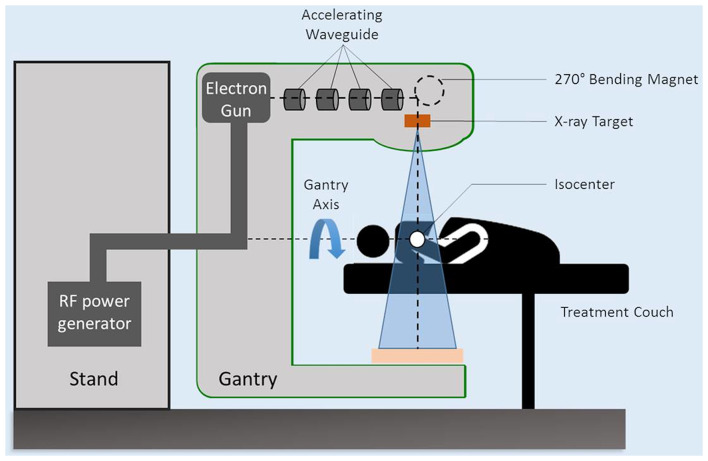
\includegraphics[width=\textwidth]{fcvm-07-00108-g0003.jpg}
    \caption{Schematic diagram of a linac \cite{Jumeau}}
    \label{fig:my_label}
\end{figure}





\subsection{Dataset}

The data used in this work will be the product of a measuring of the radiation produced by the earlier mentioned Elekta MV 6 over a water mannequin, a quite common method when it comes to radiation procedures \cite{Lutz1984-ex}, \cite{BenitesR2012}, \cite{Gonzalez2015}, \cite{Tessonnier} . The result of these measurings is a total of 96 text files, each one of these correspond to a different combination of height, area and presence (or not) of a scattering part. We can see an example of one of these profiles on Figure 2. Text files shape are as shown on table 1.


\begin{figure}[!h]
    \centering
    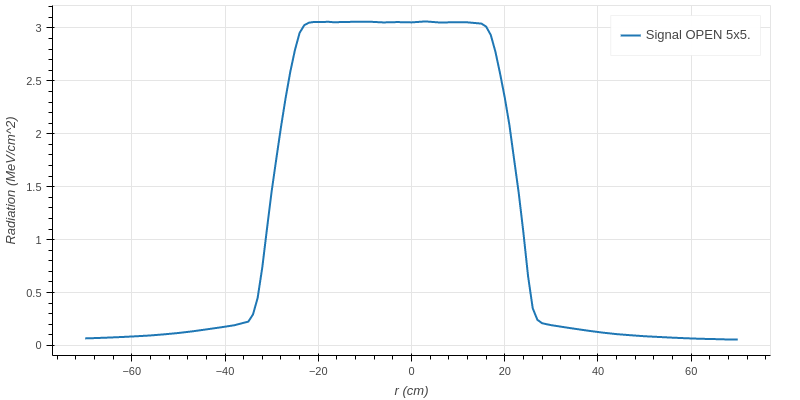
\includegraphics[width=\textwidth]{ProfileExample.png}
    \caption{5x5 open profile on y axis, z=100cm}
    \label{fig:my_label}
\end{figure}


\begin{table}[!h]
    \centering
\begin{tabular}{lrrr}
\toprule
{} &     \textbf{r} &  \textbf{señal open 5x5} &  \textbf{error open 5x5} \\
\midrule
\hline
\hline

0 & -70.0 &        0.066602 &         0.31080 \\
1 & -68.0 &        0.069431 &         0.31110 \\
2 & -65.0 &        0.074360 &         0.31065 \\
3 & -62.0 &        0.080116 &         0.31080 \\
4 & -59.0 &        0.086831 &         0.31095 \\
... & ... & ... & ... \\
70 &  59.0 &        0.067845 &         0.31395 \\
71 &  62.0 &        0.063037 &         0.31410 \\
72 &  65.0 &        0.060057 &         0.31470 \\
73 &  68.0 &        0.056351 &         0.31410 \\
74 &  70.0 &        0.055396 &         0.31410 \\
\hline
\hline

\bottomrule
\end{tabular}
\caption{Example of 5x5 profile txt}
    \label{tab:my_label}
\end{table}

\newpage 

The files in this dataset comprise of all these possible combinations:

\begin{itemize}
    \item \textbf{Area}: 5x5, 5x40, 10x10, 10x40, 20x20, 40x5, 40x10, 40x40
    \item \textbf{Z}: 85, 100, 115
    \item \textbf{FFF (scatter)}: FFF, OPEN
\end{itemize}


\newpage 

\subsection{Goals}

So, this study was focused on obtaining a Virtual Source Model for this linac based on the dataset we do have. Previous models (\cite{BenitesR2012}, \cite{Gonzalez2015}, \cite{Tessonnier}, \cite{10.1007/978-3-642-21198-0_318}, \cite{phdthesis}, \cite{https://doi.org/10.1120/jacmp.v16i1.4992}, \cite{GONZALEZ201716}) have been centered on obtaining an analytic equation that is able to mathematically define the reality. They rely on MonteCarlo or similar methods to obtain coefficients for the equation, however, this may be not the fastest nor the most effective method to obtain these results. With the current expansion of Artificial Intelligence and bayesian statistics, it may be interesting to look up those methods to solve this problem. Our objective however will be mixed. On one hand, we will obtain an analytic equation that defines our problem, obtaining the needed coefficients via MonteCarlo. \\

Once we have solved that part, we will look to improve the current result of the analytic equation feeding that data as input to several Neural Networks, which will try to create a prediction. Using Neural Networks in medical physics is not something new, as it is widely used in cancer recognition \cite{BOTTACI1997469} \cite{Ganesan} \cite{Shen2019}. However, there are not many examples of its use on dosimetry \cite{G_tz_2020} \cite{Jiang} \cite{Lee2019} and most of them are quite new. As said on Lee et al., 2019 \cite{Lee2019}, "The direct Monte Carlo simulation is considered as a state-of-art voxel-based dosimetry technique; however, it incurs an excessive computational cost and time. To overcome the limitations of the direct Monte Carlo approach, we propose using a deep convolutional neural network (CNN) for the voxel dose prediction". However, we mix both methods, trying to obtain best from both worlds.

\newpage
\numberwithin{equation}{section}

\section{Monte Carlo approximation}


Following Fippel et al (2003) \cite{Fippel} and González (2015) \cite{Gonzalez2015} VSMs, we develop one for this linac.

We can describe it as a two part equation, where the first leg of the equation corresponds to the main collimator and the second leg to the scattering. 

\begin{equation}
    \centering
    \Phi_\gamma (x,y,z) = w_0 \Phi_0(x,y,z) \Phi_{horn}^\gamma (x,y,z) + (1-w_0)\Phi_s(x,y,z) 
\end{equation}



Being more concise, \(w_0\) is the fraction of the contribution from the primary (and therefore, 1 minus \(w_0\) is the contribution from the scatter source), a normalized value. Then, \(\Phi_0\) and \(\Phi_s\) are the fluence equations for both collimator and scatter source. Finally, \(\Phi_{horn}\) is an equation that tries to define the central depression that we can see on the mayority of profiles. An example of this kind of profile can be seen on Figure 3.\\



\subsection{Photon Primary Source Fluence}

Fluence equations are defined as it follows:

\begin{equation}
    \centering 
    \Phi_\alpha = Z(z; z_D^x, z_D^y, z_\alpha) T_\alpha(x_\alpha^+, x_\alpha^-) T_\alpha(y_\alpha^+, y_\alpha^- )
    
\end{equation}

Out of these variables, Z (Eq 3.3) defines the reduction of the fluence based on the distance from the target to the source, while T defines the area. 

\begin{equation}
    \centering 
    Z(z; z^x_D, z^y_D, z_\alpha) = \frac{1}{4} \frac{(z_D^x - z_\alpha) (z^y_D - z_\alpha )}{(z-z_\alpha)^2}
    
\end{equation}

Now, T refer to x or y, depending on what axis are we on, and it is defined by Pearson VII equation (3.4). This Pearson VII equation with X and Y as subject, with \( \frac{t_0^\pm}{\delta_0}\) being \(v\), as shown on equation (3.5). So, X and Y would be defined by equations (3.6) and (3.7). 

\begin{equation}
    Q_0(v) = \frac{v}{\sqrt{1+v^2}} 
\end{equation}

\begin{equation}
    T_0 (\frac{t_0^\pm}{\delta_0}) = \frac{\frac{t_0^\pm}{\delta_0}}{\sqrt{1 + (\frac{t_0^\pm}{\delta_0})^2}}
\end{equation}


\begin{equation}
    \centering 
    X_0 = \frac{\frac{x_0^+}{\delta_0}}{\sqrt{1+\frac{x_0^+}{\delta_0}}} + \frac{\frac{x_0^-}{\delta_0}}{\sqrt{1+\frac{x_0^-}{\delta_0}}} \\
\end{equation}
\begin{equation}
    \centering 
    Y_0 = \frac{\frac{y_0^+}{\delta_0}}{\sqrt{1+\frac{y_0^+}{\delta_0}}} + \frac{\frac{y_0^-}{\delta_0}}{\sqrt{1+\frac{y_0^-}{\delta_0}}}
\end{equation}

Variables on this equation need some explanation as well. \(x_0^+\), \(x_0^-\), \(y_0^+\), \(y_0^-\) are the outer bounds that delimit the collimation area. They are defined in equation (3.8).

\begin{equation}
    t_\alpha^{\pm}  = min[\frac{w_I^tz_U^t(z-z_0) \pm 2t*z_I(z_0 - z_U^t)}{2z_I(z-z_U^t)}, \frac{w_I^tz_D^t(z-z_0) \pm 2xz_I (z_0-z_D^t)}{2z_I(z-z_D^t)}]
\end{equation}


\newpage


Now, we have finished defining new variables and these are actual data, being:

\begin{itemize}
    \item \(w_I^t\): Field size on the 'T' direction. 
    \item \(z_U^t\): and \(z_D^t\): "Up" and "Down" limits of the collimation system for x and y directions.
    \item \(z\): Position of the target on the \(z\) axis
    \item \(z_0\): Position of the main fluence source
    \item \(t\): Coordinate on x or y direction 
    \item \(z_I\): Z coordinate of the isocenter, which in this case is always 100.

    
\end{itemize}



Thereby, the photon primary source is defined in equation 3.9 (without incorporating the last leg which correspond to the central depression correction):

\begin{equation}
    \Phi_0 = \frac{1}{4} (\frac{(z_D^x - z_\alpha) (z^y_D - z_\alpha )}{(z-z_\alpha)^2})*(\frac{\frac{x_0^+}{\delta_0}}{\sqrt{1+\frac{x_0^+}{\delta_0}}} + \frac{\frac{x_0^-}{\delta_0}}{\sqrt{1+\frac{x_0^-}{\delta_0}}}) * (\frac{\frac{y_0^+}{\delta_0}}{\sqrt{1+\frac{y_0^+}{\delta_0}}} + \frac{\frac{y_0^-}{\delta_0}}{\sqrt{1+\frac{y_0^-}{\delta_0}}})
\end{equation}

However, we have not defined \(\delta_0\). This is one of the coefficients we have to find. This particular coefficient defines how abrupt is the decay from the actual fluence area to the non-fluence area.

\begin{figure}[!h]
    \centering
    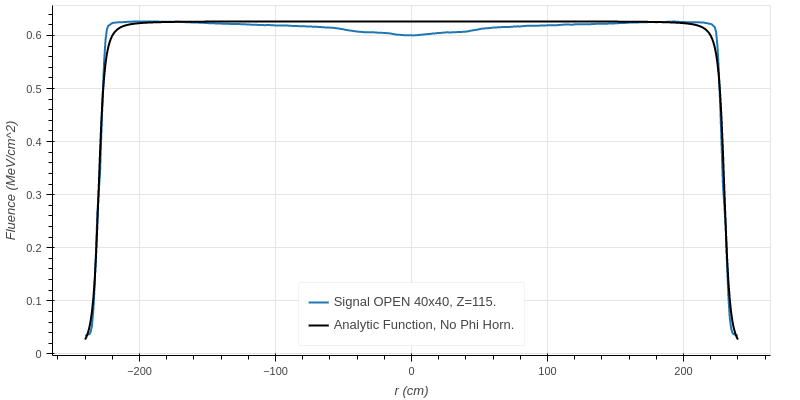
\includegraphics[width=\textwidth]{NoCentralDepression.png}
    \caption{'x' axis profile for 40x40, Z=115. Representation of the first leg of the equation vs reality using an already defined \(\delta_0\) value}
    \label{fig:my_label}
\end{figure}

\subsection{Central depression correction}

Since most profiles present a depression surrounding the center of the area, this is an added correction to the main fluence equation.

\begin{equation}
    \Phi_{horn}(x,y,z) = 1+ \rho^2 \sum_{k=0}^4 h_k \rho^k
    
\end{equation}


Where \(h_k\) are coefficients we need to obtain and \(\rho\) is a measure of the distance covered by the radiation:

\begin{equation}
    \rho = \frac{\sqrt{x^2 + y^2}}{z-z_0}
\end{equation}


The so-called central depression can be seen on Figure 4.


\begin{figure}[!h]
    \centering
    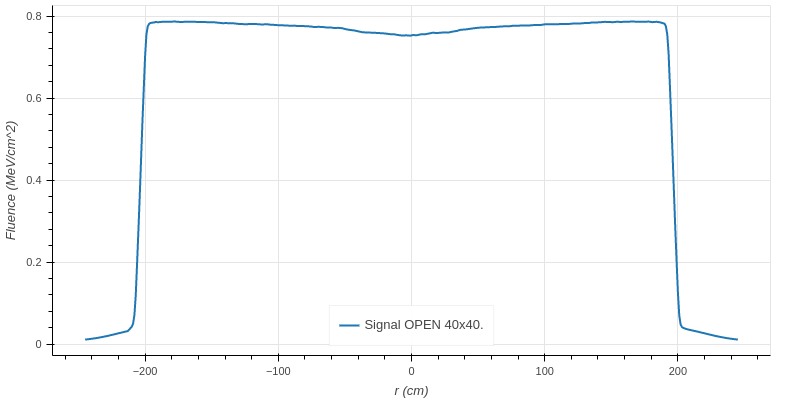
\includegraphics[width=\textwidth]{Central_Depression.png}
    \caption{'x' axis profile on the 40x40, Z=100 example. Central depression is more clear the larger the area is.}
    \label{fig:my_label}
\end{figure}




Now, in cases where we only have the main fluence source (\(w_0 = 1\)), our equation would be defined as in equation (3.12). First leg of the equation needs one coefficient, which is easily obtained, however, for the central depression correction we need 5 coefficients which is a more difficult task.

\begin{equation}
    \Phi_\gamma = \frac{1}{4} (\frac{(z_D^x - z_\alpha) (z^y_D - z_\alpha )}{(z-z_\alpha)^2})*(\frac{\frac{x_0^+}{\delta_0}}{\sqrt{1+\frac{x_0^+}{\delta_0}}} + \frac{\frac{x_0^-}{\delta_0}}{\sqrt{1+\frac{x_0^-}{\delta_0}}}) * (\frac{\frac{y_0^+}{\delta_0}}{\sqrt{1+\frac{y_0^+}{\delta_0}}} + \frac{\frac{y_0^-}{\delta_0}}{\sqrt{1+\frac{y_0^-}{\delta_0}}}) * ( 1+ \rho^2 \sum_{k=0}^4 h_k \rho^k)
\end{equation}




\subsection{Monte Carlo method}

Putting it simple, a Monte Carlo simulation \cite{Kroese2014WhyTM} is a process where we introduce random numbers as coefficients, obtaining a distribution out of them. Our desired VSM is composed at the second leg of 5 coefficients, but it is an arbitrary decision to stop at 5. We could create a more complex equation if we used more coffiecients, or less, if we used a smaller number of coefficients. As a example of this, you can see how we recreate the results using 3 coefficients (equation (3.13) and Figure 4). \\

\begin{equation}
    \Phi_\gamma = \frac{1}{4} (\frac{(z_D^x - z_\alpha) (z^y_D - z_\alpha )}{(z-z_\alpha)^2})*(\frac{\frac{x_0^+}{\delta_0}}{\sqrt{1+\frac{x_0^+}{\delta_0}}} + \frac{\frac{x_0^-}{\delta_0}}{\sqrt{1+\frac{x_0^-}{\delta_0}}}) * (\frac{\frac{y_0^+}{\delta_0}}{\sqrt{1+\frac{y_0^+}{\delta_0}}} + \frac{\frac{y_0^-}{\delta_0}}{\sqrt{1+\frac{y_0^-}{\delta_0}}}) * ( 1+ \rho^2 \sum_{k=0}^2 h_k \rho^k)
\end{equation}

\newpage 


\begin{figure}[!h]
    \centering
    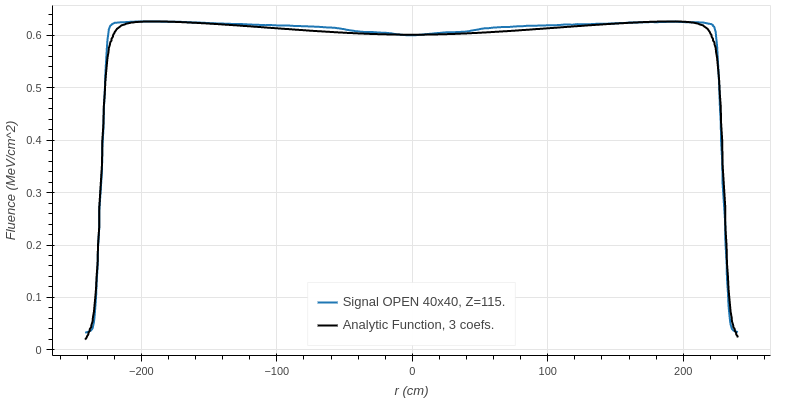
\includegraphics[width=\textwidth]{3Coefs.png}
    \caption{Signal and Analytic Function fitted using a 3 coefficient equation as \(\Phi_{horn}\). This is the plot of a case where there is no scatter signal, Z=115 and the area to be covered is 40x40 cm}
    \label{fig:my_label}
\end{figure}

VSMs on the bibliography present coefficients that are useful for both profiles ('x' and 'y'). However, during the course of this study, I realised that the behaviour of each axis was not the same, and coefficients that were good for 'x' were not so good for 'y', so it was decided to isolate each axis and study different models for each one. \\

As an example of this, if we use 'x' axis coefficients we obtained after approximately a million iterations on the 'x' axis (Table 2), we obtain a mean absolute error of \(0.0142 MeV/cm^2\). If we use the same coefficients for the 'y' axis we obtain an error of \(0.0245 MeV/cm^2\).



\begin{table}[!h]
    \centering
\begin{tabular}{lrrrrr}
\toprule
\delta_0 &     \(h_0\) &         \(h_1\)  &         \(h_2\)  &         \(h_3\)  &         \(h_4\)  \\
     \hline
\midrule
2.659 & 0.0433 &  0.0114 & -0.0383 &  0.0129 &  0.000053 \\
\bottomrule
\end{tabular}  
\caption{Best coefficients obtained for x axis}
    \label{tab:my_label}
\end{table}


These are the results obtained at the end of the iterations. However, it was clear from the beginning that profiles for both axis were different, so it was decided to search separately for each axis. \\
Monte Carlo method followed in this case was built using Python. Mayority of the calculation was run on a laptop (which has an Intel® Core™ i5-8250U CPU @ 1.60GHz × 8, a not very fast CPU in nowadays standards), the development of it was done through several batches, which would last for approximately a week.

\subsubsection{Random Monte Carlo search}

Initially, the code was meant to create random numbers between two limits for each coefficient. Since \(\delta_0\) and the 'h' coefficients are independent between them, in order to speed up the search of ideal coefficients, 'h' coefficients are searched first using an standard value of \(\delta_0\ =2\) and once found the best 'h' coefficients we do Monte Carlo again only on \(\delta_0\). Coefficients and errors were stored in lists. Each batch usually was composed of 100000 epochs, after which the results would be reviewed. Based on the lowest errors, a new iteration script would be created, adapting the limits of the random number generator for each coefficient. Initial limits were set between \(10^{-7}\) and \(10^{-1}\) for both negative and positive values. Randomization was done between '-7' and '-1' since the logarithmic scale suits better for this problem optimization. Code was similar to what is shown on appendix A. Table 3 contains results that serve as example of the first batch. 

\newpage 


Results (as shown in Table 3), show a clear pattern on the \(h_0\) coefficient. Limit was set on 1e-2, and best values surround that limit, so in the next iteration it was ideal to upgrade that limit to 1e-1 and close the bottom limit to 1-3. The other coefficients are not that clear, besides you can see that values for h and k tend to be quite low (all well below 1e-3). Color maps shown on Figures 6-9 confront \(h_0\) (which has the easiest pattern) with the other 4 coefficients, allowing us to visually check patterns. Table show as that boundaries on 'l' can been stretched a lot, while the other ones are still quite doubtful. Next batch of iterations would start on \(h_0\) limits between 1e-2 and 1e-3. Visually, we can see clear patterns on the graphics aswell, which help us to short the boundaries on the other coefficients, rather than letting the Monte Carlo method go on forever.


\begin{table}[!h]
    \centering
\begin{tabular}{lrrrrr}
\toprule
Mean Absolute Error &         l &             k &             j &             h &             g \\
\hline
\hline
\midrule
0.067715 &  0.009776 &  1.013672e-03 &  5.200028e-04 & -8.364561e-07 &  1.674677e-06 \\
0.067739 &  0.009648 &  4.834647e-03 &  2.763648e-05 & -5.879016e-04 & -1.031359e-04 \\
0.067758 &  0.008969 &  2.270703e-03 & -1.487425e-07 &  1.349939e-04 &  3.512052e-05 \\
0.067759 &  0.009235 & -7.479714e-06 &  1.295526e-03 & -2.128316e-07 & -6.476427e-06 \\
0.067791 &  0.007948 &  3.669876e-03 & -9.849719e-04 &  2.654817e-07 &  1.495117e-05 \\
0.067799 &  0.009047 & -2.627768e-04 &  3.961705e-04 &  3.323590e-04 &  5.140993e-06 \\
0.067803 &  0.009623 & -2.660140e-03 &  2.280633e-03 &  9.482199e-06 & -5.843446e-06 \\
0.067807 &  0.007860 &  5.550067e-07 & -1.400713e-05 &  8.618755e-07 &  2.529700e-04 \\
0.067811 &  0.007967 & -5.448018e-06 &  2.537317e-03 & -5.988936e-04 & -2.827558e-07 \\
0.067822 &  0.009885 & -1.369494e-06 &  1.699570e-03 &  1.661274e-06 & -4.148678e-06 \\
\hline
\hline

\bottomrule
\end{tabular}
\caption{Random search of coefficients, results after the first batch of iterations on the 'x' axis}
    \label{tab:my_label}
\end{table} \\








\begin{figure}[!h]
    \centering
    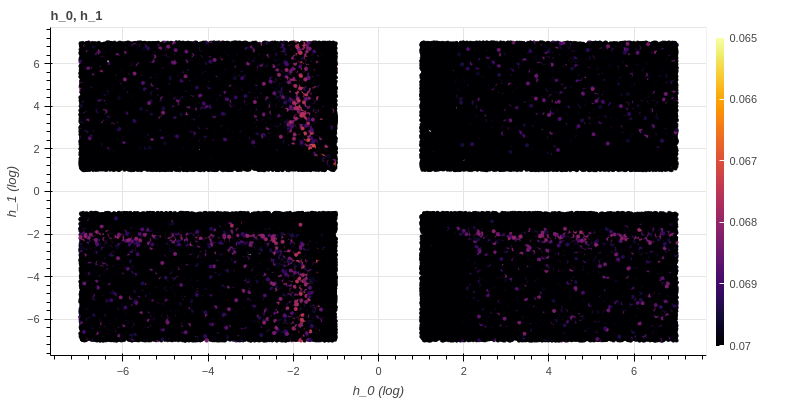
\includegraphics[width=\textwidth]{h1.png}
    \caption{\( h_0\) vs \(h_1\)}
    \label{fig:my_label}
\end{figure}

\newpage 

\begin{figure}[!h]
    \centering
    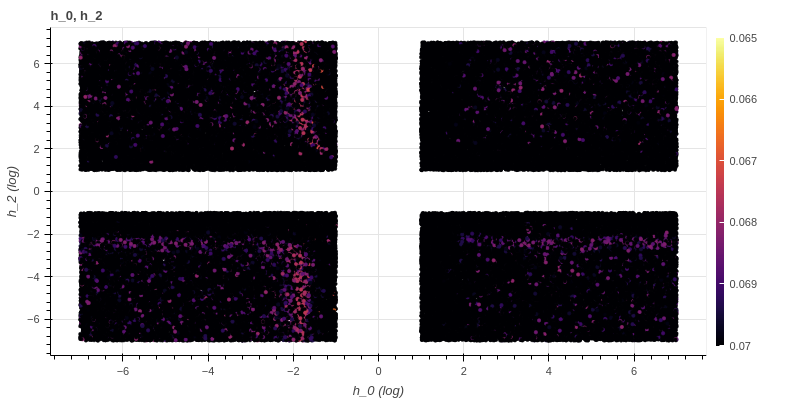
\includegraphics[width=\textwidth]{h2.png}
    \caption{\( h_0\) vs \(h_2\)}
    \label{fig:my_label}
\end{figure}



\begin{figure}[!h]
    \centering
    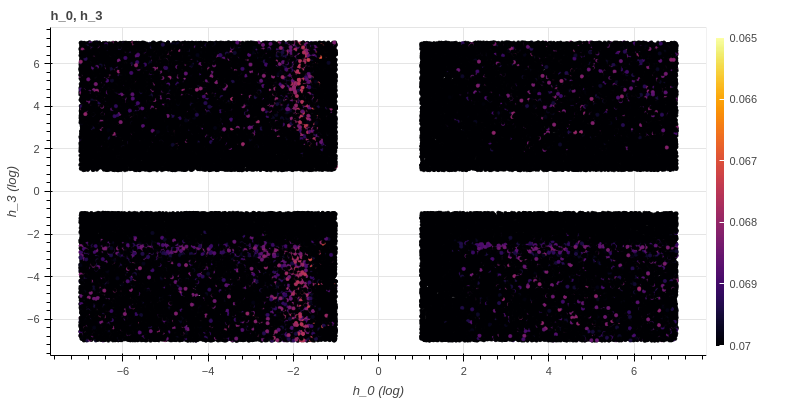
\includegraphics[width=\textwidth]{h3.png}
    \caption{\( h_0\) vs \(h_3\)}
    \label{fig:my_label}
\end{figure}

\newpage 

\begin{figure}[!h]
    \centering
    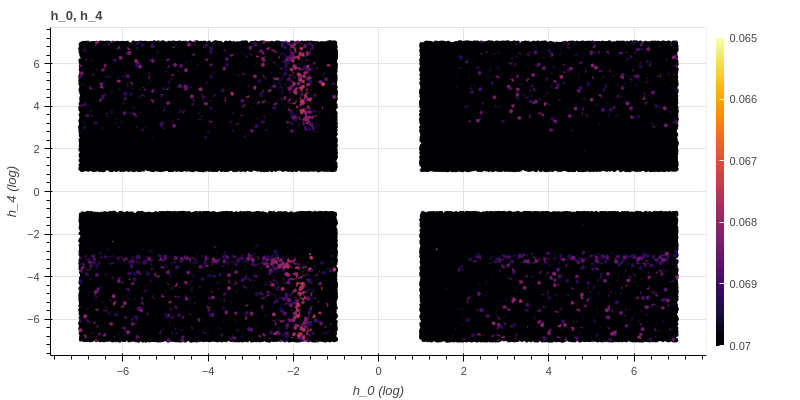
\includegraphics[width=\textwidth]{h4.png}
    \caption{\( h_0\) vs \(h_4\)}
    \label{fig:my_label}
\end{figure}





\subsubsection{Non randomized Monte Carlo method}

Besides the pure Monte Carlo method is meant to be totally random, the presence of 5 coefficients, the selection of python as engine (high-level, interpreted language, easy to use but not very efficient resource-wise) and lack of powerful hardware makes it difficult to achieve a great result using pure randomness. So, it was decided to create a set of given variables (10 possibilities, 5 negative and 5 positives, growing on a logarithmic way from \(10^{-7}\) to \(10^{-1}\)) and try all the possible combinations between them. This method allowed us to obtain more clear results in a faster way. Table 4 shows results for first batch of iterations on x axis using non randomized way (and their coefficients). On Figure 10 we can see a comparative error distributions for first iteration (100000 trials) for both methods. Both methods achieve quite similar results, with the randomized one obtaining slightly better error on its peak, but the non randomized method offers an easier look at what are the best combinations. Since we are not looking for the best overall result (since this is the first iteration of many to come), the objective of the iterations at this point is to set the next limits. This s better achieved through the non randomized method, which is followed for the rest of the study.

\begin{table}[!h]
    \centering
\begin{tabular}{lrrrrr}
\toprule
\textbf{Error} &       \textbf{\(h_0\)} &           \textbf{\(h_1\)} &       \textbf{\(h_2\)} &           \textbf{\(h_3\)} &    \textbf{\(h_4\)} \\
\midrule
\hline
\hline 
0.068006                &  0.003162 &  3.162278e-03 &  1.000000e-04 &  0.0001 &  0.000100 \\
0.068040                &  0.003162 &  3.162278e-03 &  3.162278e-06 &  0.0001 &  0.000100 \\
0.068042                &  0.003162 &  3.162278e-03 &  1.000000e-07 &  0.0001 &  0.000100 \\
0.068042                &  0.003162 &  3.162278e-03 & -1.000000e-07 &  0.0001 &  0.000100 \\
0.068043                &  0.003162 &  3.162278e-03 & -3.162278e-06 &  0.0001 &  0.000100 \\
0.068063                &  0.003162 &  3.162278e-06 &  3.162278e-03 & -0.0001 & -0.000003 \\
0.068063                &  0.003162 &  1.000000e-07 &  3.162278e-03 & -0.0001 & -0.000003 \\
0.068063                &  0.003162 & -1.000000e-07 &  3.162278e-03 & -0.0001 & -0.000003 \\
0.068063                &  0.003162 & -3.162278e-06 &  3.162278e-03 & -0.0001 & -0.000003 \\
0.068064                &  0.003162 &  1.000000e-04 &  3.162278e-03 & -0.0001 & -0.000003 \\
\bottomrule
\hline
\hline 

\end{tabular}
    \caption{Best results obtained on the non-randomized Monte Carlo}
    \label{tab:my_label}
\end{table}
\newpage 

\begin{figure}[!h]
    \centering
    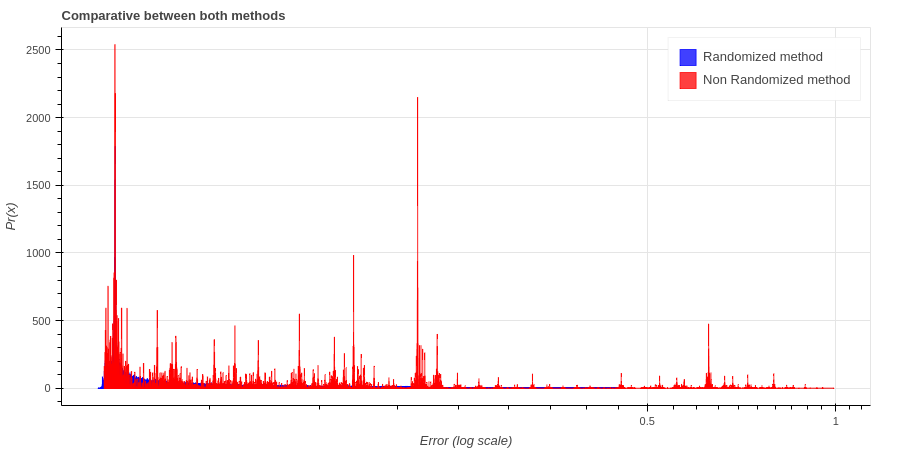
\includegraphics[width=\textwidth]{Comparative_Random_NONRandom.png}
    \caption{Histograms showcasing error for both methods}
    \label{fig:my_label}
\end{figure}




\newpage 


\section{Artificial Intelligence}

\subsection{Introduction}

Science by definition is a way of mathematizing reality, the study and work that tries to represent reality in an organized and predictable way. However, problems on reality are not isolated like they are on laboratories and the attempts to predict in a scientific way any kind of 'open' problem is just an approximation. This is esentially the case here. Besides the trials are made on a laboratory, there are variables that we cannot take into account. In this case, we have already seen that profiles on the x axis are not exactly the same than profiles on the y axis, and there are some drops in different zones. Those are problems that come with the machine we are using, and they will replicate, but obtaining analytical approximations that define these problems is a kind of study that would take tremenduous work for not so much reward. That is a great point for the use of Artificial Intelligence on Science, it does not substitute the equations, they simply work as a way of smoothing and approximating results when the work needed to achieve a significant improvement is not worth, which is the main part of this study.\\

Artificial Intelligence (AI from now on), is a broad concept that unites several fields. Monte Carlo method for example is also defined as AI, since usually, AI is defined as a computerized way of applying statistics and maths on a automatized way. AI development in the last 50 years has gone through 3 eras (\cite{8259629}, \cite{BINI20182358}):

\begin{itemize}
	\item Artificial Intelligence: Primitive AI, automatized statistics and maths, Monte Carlo method is a classic example of this field. However, following development is still included as AI.
	\item Machine Learning: First proper development of what AI is usually understood as. Examples of this field are Tree Decision algorithms (\cite{palmer1979number}, \cite{batra1975classification}) and Gradient Boosters \cite{FREUND1997119}.
	\item Deep Learning: Neural Networks on all its variaties
\end{itemize}

On the previous section we have defined what Monte Carlo method is, so there is no need for further introduction. However, Machine Learning and Deep Learning will be introduced as they were both used for this project.

\subsection{Machine Learning}

There was no doubt of the utilities of basic AI, so, the first steps after classic AI were moved towards developing automatized AI that needed less information from the user, keeping the iterative algorithm that tries to solve problems. There came Random Forests (decision trees algorithms) and Gradient Boosters. For classic AI, like Monte Carlo, we define an equation and try different coefficients. There are different ways to develop it, using random sets of data, randomizing only per coefficient, using given sets of data, etc. but in all cases you need a defined equation. First big difference with machine learning (ML from now on): it does not need an equation. ML needs a 'x' array and 'y' array. 'x' array correspond to the number of variables we have, and 'y' is the result we are trying to achieve (Equations 4.1, 4.2). Sets of data are usually divided in two, a training dataset from which the algoritm tries to learn the correlations, and then it is validated on a test/validation dataset. If we tried to obtain a result out of machine learning for our case, we could use all 'x' variables we have for each 'y', without producing a proper equation earlier. In our case, each single point on the dataset is randomly assigned to either training or validation (on a 75-25\% proportion).  \\

\newpage 


\begin{equation}
\centering 
\left(
\begin{array}{c}
     x_0^0 \\ 
     x_1^0 \\ 
     x_2^0 \\
     ... \\
     x_n^0 
\end{array}
\right) \rightarrow y^0 \\


\end{equation}

Machine learning work iterating through multiple samples, until it obtains the combination of operations and coefficients that approach the most to the desired results.

\begin{equation}

\centering
\left(
\begin{array}{ccc}
     x_0^0 & ... & x_0^t \\ 
     ... & ... & ... \\
     x_n^0 & ... & x_n^t 
\end{array}
\right) \rightarrow \left(\begin{array}{ccc}
    y^0 & ... & y^t \\
\end{array}\right)


\end{equation}




Here, ML algorithms (Figures 11, 12), try to obtain a correlation between those variables and fluence. However, it does not work out great. ML presents a problem, it work looking for simple correlations. In other words, they do not understand arrays as a whole cohesive set of data, but single points. In our case, this is key, fluence for each single point is not defined individually, we are looking to obtain the complete figure of the fluence profile, and using singular data is not enough, since each point has an structural relevance.

\newpage 

\begin{figure}[!h]
    \centering
    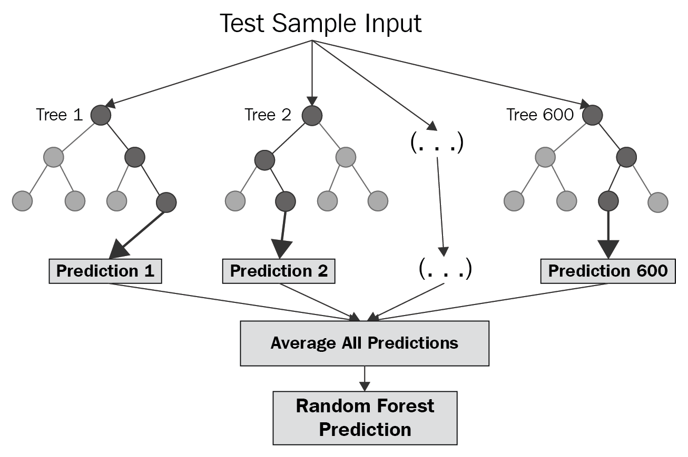
\includegraphics[width=\textwidth]{random-forest.png}
    \caption{Random Forest schema. It works as a decision tree, averaging results from every tree at the end of the process}
    \label{fig:my_label}
\end{figure}

\begin{figure}[!h]
    \centering
    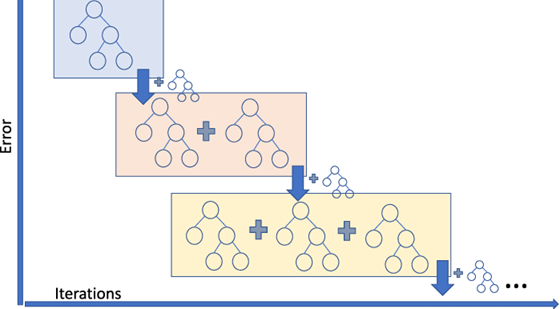
\includegraphics[width=\textwidth]{Gradient Boosting.png}
    \caption{Gradient Boosting schema. It works similar to a random forest, but instead of averaging results at the end, each tree is made out of a previous one for each iteration, this way doing a 'real time' average}
    \label{fig:my_label}
\end{figure}


\newpage 


\subsection{Deep Learning}

So, latest installment of AI is Deep Learning (DL). DL adresses previously mentioned problems, they are able to understand complete arrays as data, using data in more than 2 dimensions iterating until it obtaines the best possible result. The biggest improvement on this line of work can be seen easily on matters like image detection. ML works on flattened 2-dimension arrays. So, in order to apply this to image classification, how could you work it out? You would have to convert 3-dimension arrays (height, width, number of channels hannels) to a 1-dimension array, stacking height, width and number of channels (if an image is RGB, is composed of 3 different channels), obtaning a number of variables (height*width*number\_channels) = (result). Each pixel would be a variable. If we converted that array back to an image, we would have an image of height 1 and width equal to the total number of pixels there is in the image. This may be hard to comprehend but on figures 13 and 14 \cite{Dog} the example is self-explanatory.

\begin{figure}[!h]
    \centering
    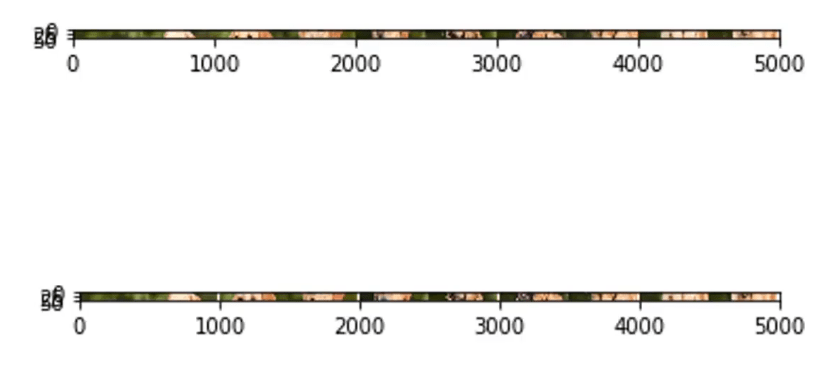
\includegraphics[width=0.8\textwidth]{FlattenedImage.png}
    \caption{These are two images of dogs, flattened arrays as ones that a ML algorithm can read, one of them is true and the other has been modified}
    \label{fig:my_label}
\end{figure}

\begin{figure}[!h]
    \centering
    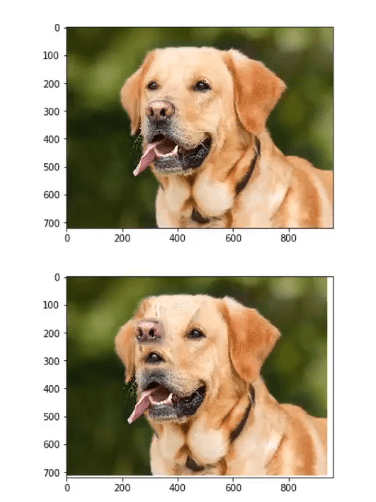
\includegraphics[width=7cm]{NonFlattenedDog.png}
    \caption{These are the same pictures showed on Figure 12. A simple demostration of how important the spatial configuration of an array may be}
    \label{fig:my_label}
\end{figure}


However, DL solves that problem and allow us to feed algorithms using other kind of dimensions. Probably the two most used Neural Network types are 'LSTM' (Long Short Term Memory) Neural Networks \cite{LSTM} and CNN (Convolutional Neural Networks) \cite{DBLP:journals/corr/OSheaN15}. \\
LSTMs are ideal for sequencial timeline-related data, they are fed with 3-dimension arrays, where each point is a time step. These kind of models are designed to learn that time steps are correlated, and, variables effect to a result on a time 't' are more related to how variables affected to a result on a time 't-1' than how variables affected to a result on 't-500'. \\
CNNs are ideal to image, video, or audio classification, because they understand arrays as a whole. A visual example: if we convert a set of videos to arrays we obtain a 5-dimensional array (number of samples, height, width, number of channels, time). The coherence between each one of those dimensions is key, and it is something not possible to achieve using ML or classic AI.

CNNs have 3 main types:

\begin{itemize}
	\item Conv1D: 1 added dimension to a simple array. Examples: Audio signals (3 dimensions)
	\item Conv2D: 2 added dimensions to a simple array. Examples: Pictures (4 dimensions) 
	\item Conv3D: 3 added dimensions to a simple array. Examples: Video (5 dimensions)
\end{itemize}

Our problem is not a video , but we could compare it with an audio signal. Profiles have much in common between them and some variables make them change, but out of data exploration we can see easily that they should be understood as a whole. We can adress that kind of problem with Conv1D NN. Our data may be presented as shown on equation 4.3 (assuming n varibles, m samples and a width for each profile that goes from -r to r). \\

\begin{equation}
        \centering
    \left(\begin{array}{c}
\left(
\begin{array}{ccc}
     x_0_,_{-r} ^0 & ... & x_0_,_{-r}^n \\ 
     ... & ... & ... \\
     x_0_,_{r}^0 & ... & x_0_,_{r}^n 
\end{array}
\right)  \\
\\\
\left(
\begin{array}{ccc}
     x_1_,_{-r} ^0 & ... & x_1_,_{-r}^n \\ 
     ... & ... & ... \\
     x_1_,_{r}^0 & ... & x_1_,_{r}^n 
\end{array}
\right)

\\\
\\
...
\\\
\\
\left(
\begin{array}{ccc}
     x_m_,_{-r} ^0 & ... & x_m_,_{-r}^n \\ 
     ... & ... & ... \\
     x_m_,_{r}^0 & ... & x_m_,_{r}^n 
\end{array}
\right)
\end{array}\right) \rightarrow \left(\begin{array}{c}
     \left(\begin{array}{c} y_0,_{-r} \\
     ...\\
     y_0,_r \end{array}\right)  \\
     \\\
     
     \left(\begin{array}{c} y_1,_{-r} \\
     ...\\
     y_1,_r \end{array}\right) \\
     \\\
     ... \\
    \\\
     
     \left(\begin{array}{c} y_m,_{-r}\\
     ...\\
     y_m,_r \end{array}\right)
\end{array}\right)
\end{equation}\\

Here, another small problem appear for us. Data fed to the Neural Networks must have always the same shape, something that it does not happen in our case, since data for each profile only cover the parts of the data where there is significant signal, plus a few centimeters more. Therefore, profiles on the 5x5 area have way less 'width' than the 40x40 profiles. To solve that problem, we 'resample' data, obtaining the mean value for each point (this resample is done obtaining data for each 0.5cm). If there is no value surrounding that point, we interpolate the data through a polynomial equation, and limits of the data are set as the minimun value obtained.




\newpage

\section{Modelization}

\subsection{Settings}

So, once we know that we are using Conv1D Neural Networks, we need to create that model. While ML or AI do not need much configuration, with the complexity of Neural Networks comes a way higher amount of configuration possibilites. Some of them may be known from theoretical knowledge, but many of them need to be tried before discarded. Neural Networks may be created manually, since they are basically a iterator that uses certain activation functions, but it is easier to use predefined frameworks created from the main software companies of the world. Both Meta and Google have their own branches of DL. Tensorflow (Google) \cite{45381} is the most broadly used DL framework nowadays and will be the one that we will be using on this project. \\

Base CNN model is composed of a number of entry convolutional layers that usually increase periodically the number of filters they are applying, which then get translated to 'Dense' (also called 'MLP', Multi Layer Perceptron) layers, which are a type of layer that work similar to ML. We will use 3 Convolutional layers linked to 3 Dense layers. The list of settings (which will be further explained later) to configure is:

\begin{itemize}
	\item Number of filters on Convolutional layers 
	\item Kernel size on Convolutional layers
	\item Number of neurons on layer 4 (Dense)
	\item Number of neurons on layer 5 (Dense)
	\item Activation function on layer 1 (Conv1D)
	\item Activation function on layer 2 (Conv1D)
	\item Activation function on layer 3 (Conv1D)
	\item Activation function on layer 4 (Dense
	\item Activation function on layer 5 (Dense)
	\item Activation function on layer 6 (Dense
	\item Dropout
	\item Optimizer
	\item Loss function

\end{itemize}

Iterator code is shown on appendix C and will be further explained now.

\subsection{Hyperparameter tuner}

In order to obtain the best possible configuration, we use a tool called keras tuner \cite{omalley2019kerastuner}. Tensorflow is the DL engine used, while keras is the framework that works as frontend for Tensorflow, both developed by Google. Keras tuner is an iterator that may go through 3 methods (Random Search, Bayesian Optimization or Hyperband) to try different combination of the selected hyperparameters (the previously mentioned settings to configure).

\begin{itemize}
    \item Random Search: a pure random search that combines selected settings in any possible way, keeping the best result
    \item Bayesian Optimization: It starts the iterations using random combinations. Once it gets results out of these combinations, it starts choosing new combinations based on the previous results, discarding the settings that did not work earlier, iterating until the chosen maximun number of trials. 
    \item Hyperband \cite{JMLR:v18:16-558}: This model tries several predefined configurations based on previous studies, iterating over early stops. On other words, if you want a certain Neural Network to iterate for 60 epochs, this iterator model will start iterating over just 2 or 4 epochs, comparing different configurations and developing further only the ones that present good results. This method is an order of magnitude faster than Bayesian Optimization, obtaining similar results, so it was the used method for this study.
\end{itemize}


\subsection{Hyperparameters}

\subsubsection*{Filters}

Dimension space of our data after it has gone through the convolutional layer.

\begin{figure}[!h]
    \centering
    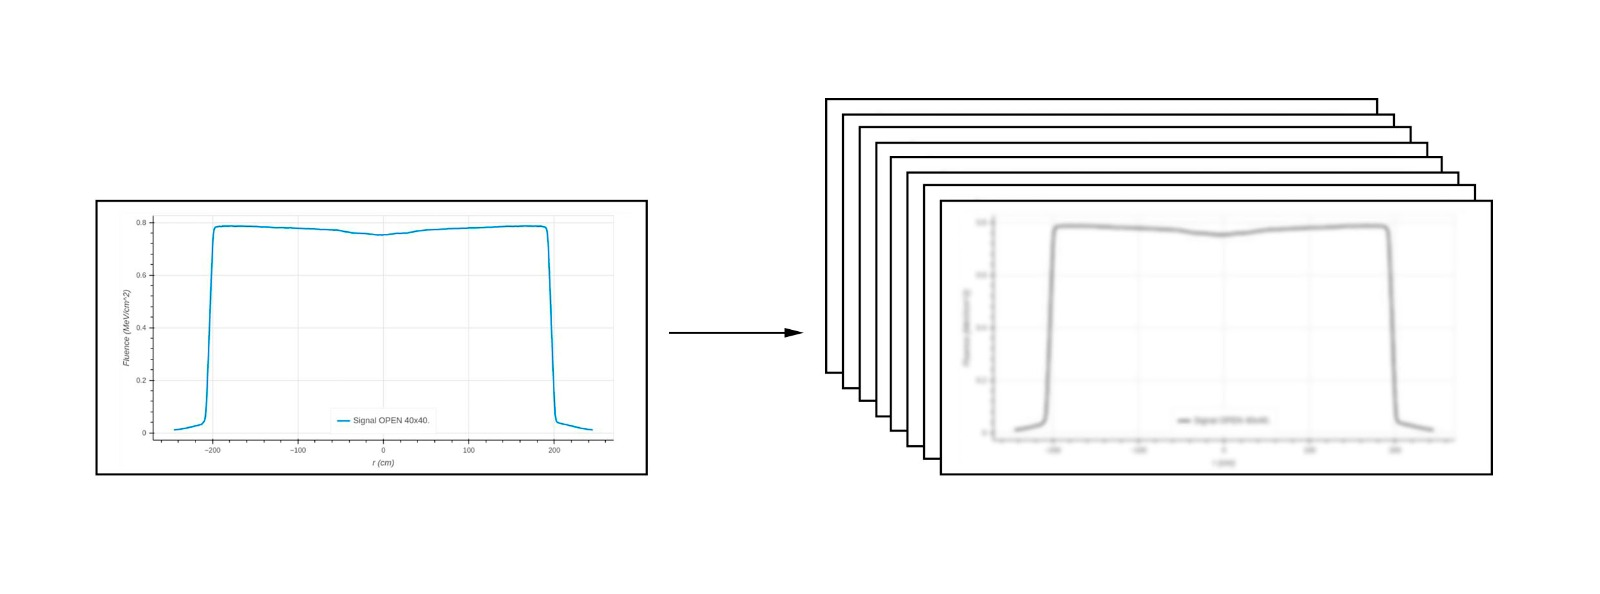
\includegraphics[width=0.8\textwidth]{Filters.jpeg}
    \caption{Schematic representation of convolutional network layers. In this case we would have 8 filters, which is a pretty common number, normally, convolutional layers are stacked in geometric progressions of 2.}
    \label{fig:my_label}
\end{figure}

\subsubsection*{Kernel}
Convolutional layers go through the data learning in batches. When we are using one-dimensional data, kernels have one dimension as well

\begin{figure}[!h]
    \centering
    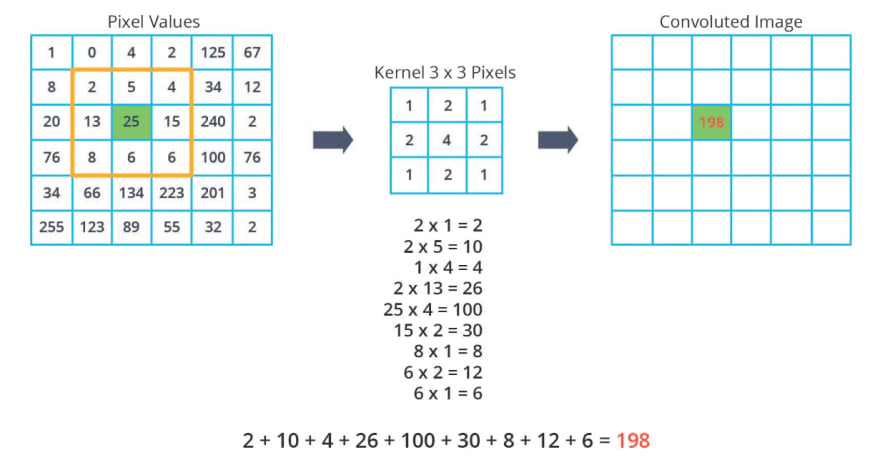
\includegraphics[width=\textwidth]{Kernel.png}
    \caption{Besides we are using 1D kernels, it is easier to understand examples with 2D kernels like the one on this figure}
    \label{fig:my_label}
\end{figure}

\subsubsection*{Activation function}

Non linear functions that allow linear information processed from one layer proceed to the next layer \cite{sharma2017activation}. On regression problems like the ones we are facing, 'relu' and its derivates are the best options, so we kept 3 possibilites: Relu (5.1), elu (5.2) and selu (5.3). On the mid layers we use those 3 layesr, while on the output layer we may use 'relu' or 'linear' (which means there is no activation function and we obtain a linear result as result of the last layer).



\begin{multicols}{3}
\begin{equation}
\centering
    \begin{cases}
    0 & \text{if } x < 0\\
    x & \text{if } x \geq 0
\end{cases}
\end{equation}\break
\begin{equation}
    \begin{cases}
    \alpha(e^x - 1) & \text{if } x < 0\\
    x & \text{if } x \geq 0
\end{cases}
\end{equation}\break
\begin{equation}
    \lambda \begin{cases}
    \alpha(e^x - 1) & \text{if } x < 0\\
    x & \text{if } x \geq 0 
    \end{cases}
\end{equation}
\end{multicols}

With \(\lambda = 1.0507\) and \(\alpha = 1.67326\) for Selu and \(\alpha\) to be found on Elu.


\begin{figure}[!h]
    \centering
    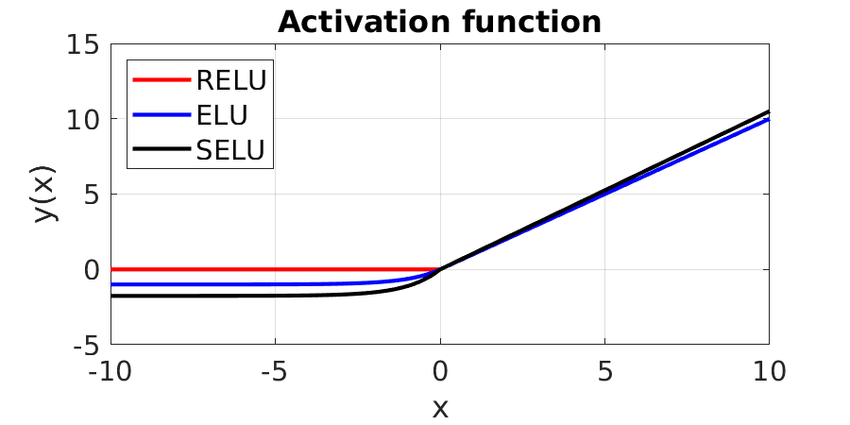
\includegraphics[width=0.7\textwidth]{Activations.png}
    \caption{Graphic representation of our activation functions}
    \label{fig:my_label}
\end{figure}

\subsubsection*{Neurons}

Number of neurons on a layer, similar concept than filters, but in this case the spatial dimension is diferent, and they are named this way for 'Dense' (MLP) layers.

\begin{figure}[!h]
    \centering
    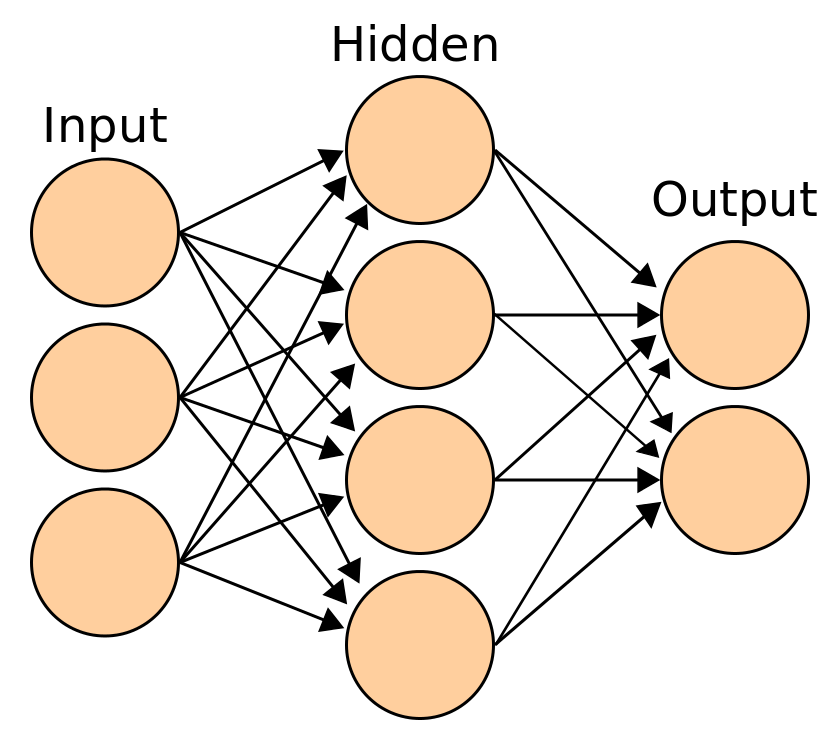
\includegraphics[width=7cm]{neurons.png}
    \caption{Really basic scheme of a NN. Input layer is defined by the dimension of our data, hidden layer is the actual number of neurons we have to define and output is the dimension we want as output (in our case, 1) }
    \label{fig:my_label}
\end{figure}

\subsubsection*{Dropout}

Percentage of the neurons not used in each epoch of the model. This is made to avoid overfitting, this way neurons will learn assimetrically in a temporal matter, so the results don't converge so fast and converge from different angles.

\subsubsection*{Optimizer}

The type of algorithm used to evolve the weights ('coefficients') through every epoch and what speed that evolution is made (learning rate). You can also set an initial learning rate, but in this case we not done that, sticking with the standard learning rate for each optimizer and allowing it to evolve naturally. We try 3 types on this example, RMSprop \cite{RMSprop}, Adam (algorithm obtained as a kind of combination of RMSprop and Adagrad \cite{duchi2011adaptive}) and Adamax (which is basically an Adam modification using infinite 'p') \cite{Adam}. Optimizers look to minimize error, reaching a global minimum. A classic problem on Deep Learning is setting the learning rate in a proper way to not get stuck on a local minimum, that's why these optimizers and their evolving learning rate are so important. We can picture this on Figure 19 \cite{gradient}.

\begin{figure}[!h]
    \centering
    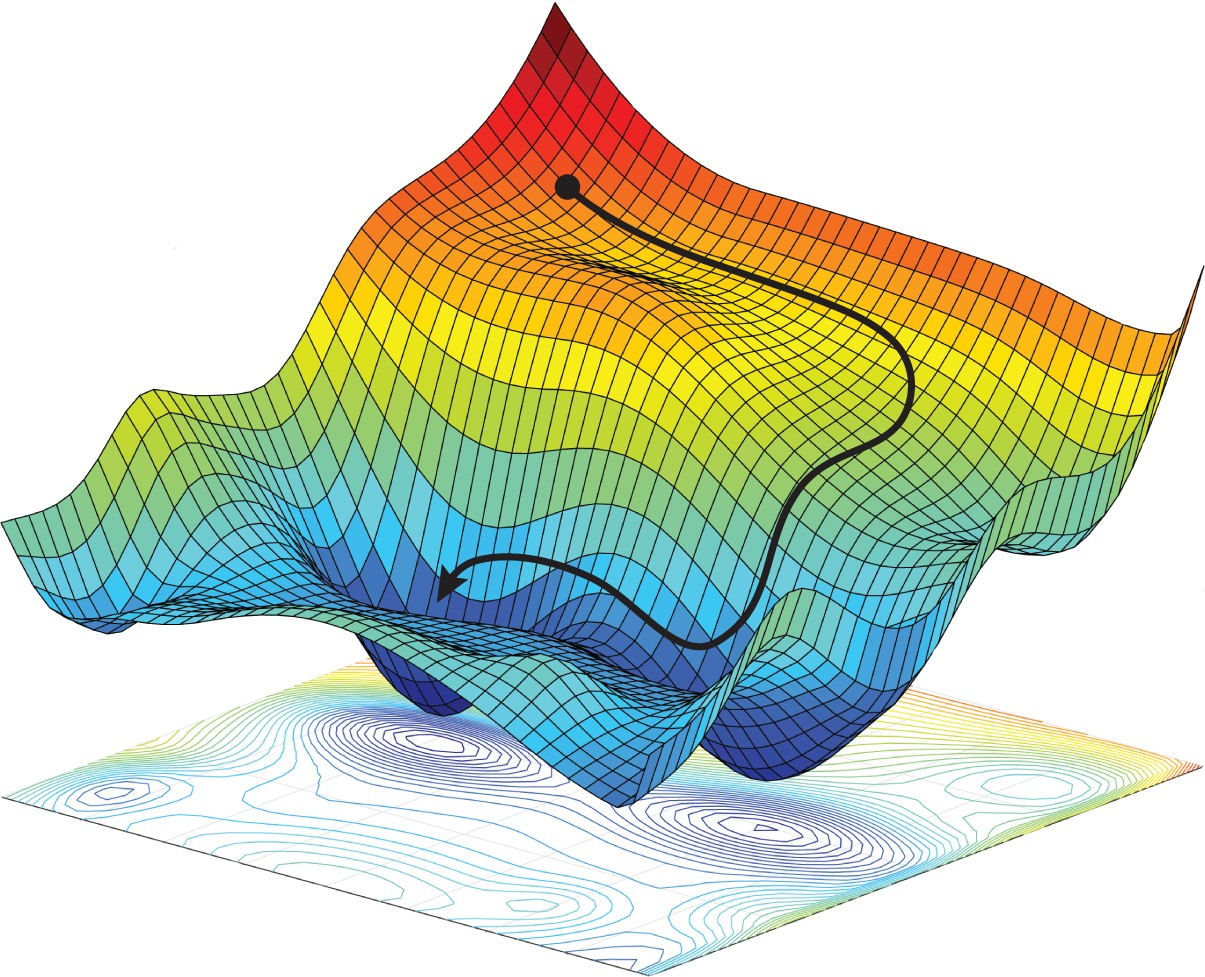
\includegraphics[width=0.8\textwidth]{LRMinimun.png}
    \caption{Schematic figure of the evolution of Neural Networks results. Picture tries to recreate the evolution of weights (black arrow) going back and forth. Color and height represent loss measure, we can see how the Neural Network finds a local minimum. However, keeps searching and after increasing error for while finds the global minimum. }
    \label{ig:my_label}
\end{figure}

\begin{itemize}
    \item Adam
    
    \item Adamax
    
    \item RMSprop
    
\end{itemize}

\subsubsection*{Loss function}

Neural Networks iterates the previously mentioned algorithms looking to minimize a loss function. Loss functions for regressions cases are usually Mean Absolute Error (MAE) and Mean Squared Error (MSE). In this case we add a function called logarithm of the hyperbolic cosine (log\_cosh), which approximates very much to mean squared error but is less affected by outliers, obtaining an overall better results if there are many outliers.

\begin{itemize}
    \item MAE
    \begin{equation}
        Loss = \sqrt{|Prediction-y_{test}|}
    \end{equation}
    \item MSE
    \begin{equation}
        Loss = |Prediction-y_{test}|
    \end{equation}
    \item log(cosh(f(x))
    \begin{equation}
        Loss = log(\frac{e^x + e^{-x}}{2})
    \end{equation}
\end{itemize}

As an example of how useful may log(cosh(f(x)) be compared to MAE can be seen on Figure 20.

\begin{figure}[!h]
    \centering
    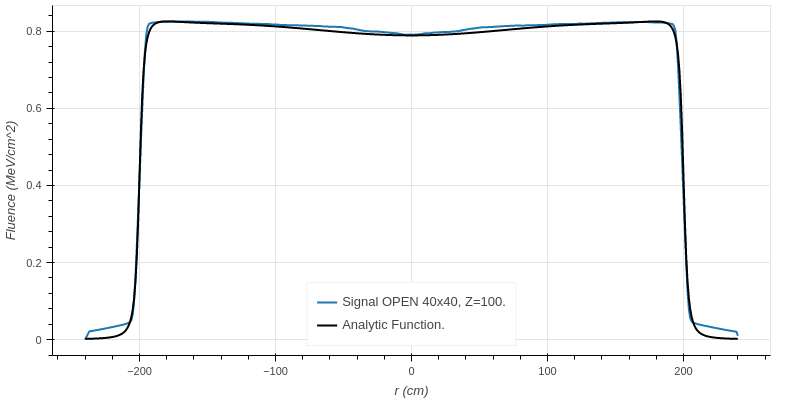
\includegraphics[width=\textwidth]{Outlier example.png}
    \caption{Monte Carlo result in contrast to original data for the 40x40 no scattering x profile, Z=100}
    \label{fig:my_label}
\end{figure}

We can see that both arms of the profile present big outliers, since the equation turn the result close to 0 after the defined zone is over, while the actual data present that there are some fluence leftovers. We cannot achieve to solve those leftovers using none of our coefficients. 'h' coefficients refer to the central depression, while the \(\delta_0\) coefficient refer to how abrupt the slope is, which we can see that are quite well fitted. However, MAE loss will be relatively high due to those outliers, and when the Neural Network tries to solve the problem and minimize the loss, if we used MAE, it might worsen the result on the fluence zone while improving the outliers. Using log(cosh) we can solve this particular problem, improving the overall result while not overfitting on the outliers. 

\newpage 

\subsection{Input data}

Normally, a neural network problem is composed of several 'x' variables that compose a sort of equation, like we mentioned earlier. On this case the inmediate variable we want to use as input for the neural network is the VSM that we developed through Monte Carlo. There are other variables that may help us (some of them mentioned earlier on subsection 3.1 Photon Primary Source Fluence).


\begin{itemize}
    \item \(w_I^t\)
    \item \(z_U^t\)
    \item \(z\)
    \item \(t\)
    \item \(z_I\)
    \item \( \rho \)
\end{itemize}

Information obtained through these variables is a bit redundant (for example Z and t are correlated to Rho). To adress that and clean data, we use Principal Component Analysis (PCA) \cite{tipping1998mixtures}. This mathematical method comprises data on a lower dimentional space. That is, if you have a 280x6 array, you can transform it into a 280x2 shaped array for example. That is one of the methods, selecting a desired shape. The other method, which we will use, is comprising a \% of the information on the data in the lowest shape possible. We use a 99\% data conservation for our case.\\
\\
Showing a visual representation of this process is not easy since representation of more than 3 dimension is not really comprehendable for human perception, but we can show a simpler example with 2 of those variables 

\begin{figure}[!h]
    \centering
    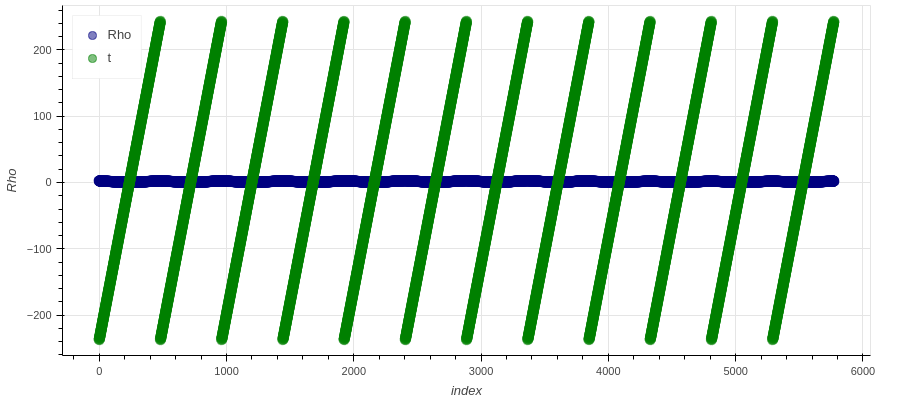
\includegraphics[width=\textwidth]{PrePCA.png}
    \caption{'t' and 'Rho' representation for all our data, horizontally stacked (index represent each one of the values for all singular cases)}
    \label{fig:my_label}
\end{figure}

\begin{figure}[!h]
    \centering
    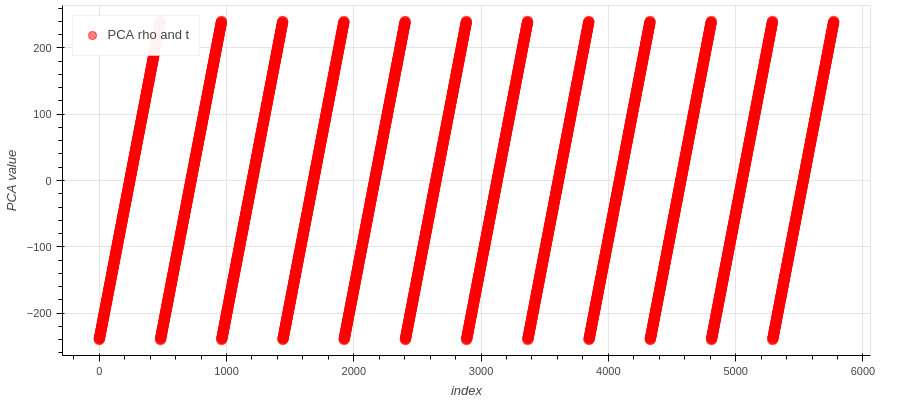
\includegraphics[width=\textwidth]{PCA.png}
    \caption{Representation of the new variable obtained by PCA. It is really similar to 't' value,  but it is not exactly the same. On this particular case, 99.997266 \% of the information was kept after the PCA was done.}
    \label{fig:my_label}
\end{figure}

\newpage 

For further clarification, if we obtain the difference between t and the PCA result, we obtain Figure 23, which is really similar to the visual representation of \(\rho\) on figure 24 (although it is in a different scale, which is the pursued point). 

\begin{figure}[!h]
    \centering
    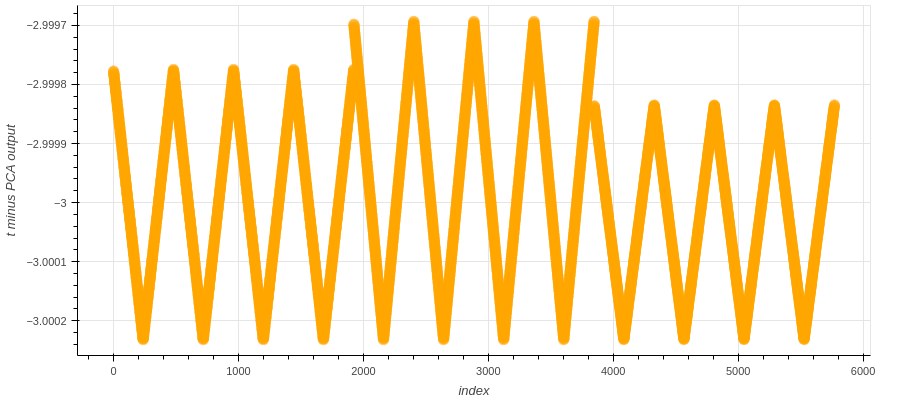
\includegraphics[width=\textwidth]{PCA-T.png}
    \caption{PCA minus T}
    \label{fig:my_label}
\end{figure}


\begin{figure}[!h]
    \centering
    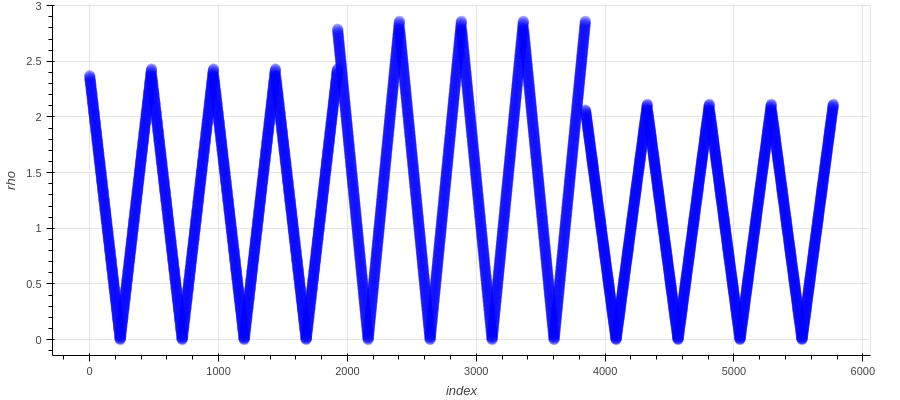
\includegraphics[width=\textwidth]{Rho.png}
    \caption{Rho values}
    \label{fig:my_label}
\end{figure}

\newpage 

After PCA is applied, data meant to be used on Neural Networks (or in general, IA algorithms) are usually normalized \cite{589532}. This operation speeds up computing of the results (lower number are easier to manipulate by the process) and usually improves results. If we apply PCA to all external variables (except our analytic function obtained through Monte Carlo) before normalizing, we end up having a 5772x2 matrix. If we apply PCA after applying normalization to said values, we obtain a 5772x5 matrix. To feed to the Neural Network we try three sets of data.

\begin{itemize}
    \item PCA of extenral variables and then normalization of output and Analytic Function
    \item Normalized analytic function
    \item Normalization of external variables, PCA and then normalized PCA output and normalized  analytic function as data
\end{itemize}




\newpage 

\section{Results}

\subsection{Monte Carlo results}

Due to the previously mentioned hardware and software limitations, results have not been equal to both axis. Also, due to the desired delivery dates, there was not enough time to get the same number of iterations for x and y profiles. However, both results are fine enough to get an approximation and to confirm our method (using them as input for a Neural Network).

\subsection{}

\newpage

\newpage

\section{Conclusions}

\newpage

\newpage


\newpage

\printbibliography




\newpage
\appendix

\section{Monte Carlo}

\subsection{Random Monte Carlo}

\begin{minted}{python}


error = []
usedl = []
usedk = []
usedj = []
usedh = []
usedg = []

for i in range(0, 100000):
    l = float(random.choices([-1, 1])[0])*10**(np.random.uniform(low=-7, high=-1))
    k = float(random.choices([-1, 1])[0])*10**(np.random.uniform(low=-7, high=-1))
    j = float(random.choices([-1, 1])[0])*10**(np.random.uniform(low=-7, high=-1))
    h = float(random.choices([-1, 1])[0])*10**(np.random.uniform(low=-7, high=-1))
    g = float(random.choices([-1, 1])[0])*10**(np.random.uniform(low=-7, high=-1))


...

    error.append(momerror)
    usedl.append(l)
    usedk.append(k)
    usedj.append(j)
    usedh.append(h)
    usedg.append(g)

\end{minted}

\subsection{Directed Monte Carlo}

\begin{minted}{python}


error = []
usedl = []
usedk = []
usedj = []
usedh = []
usedg = []

ls1 = 10**np.linspace(-1, -7, 5)
ls2 = -10**np.linspace(-1, -7, 5)
ls = np.hstack([ls1, ls2])

ks1 = 10**np.linspace(-1, -7, 5)
ks2 = -10**np.linspace(-1, -7, 5)
ks = np.hstack([ks1, ks2])

js1 = 10**np.linspace(-1, -7, 5)
js2 = -10**np.linspace(-1, -7, 5)
js = np.hstack([js1, js2])

hs1 = 10**np.linspace(-1, -7, 5)
hs2 = -10**np.linspace(-1, -7, 5)
hs = np.hstack([hs1, hs2])


gs1 = 10**np.linspace(-1, -7, 5)
gs2 = -10**np.linspace(-1, -7, 5)
gs = np.hstack([gs1, gs2])



for l in ls:
    for k in ks:
        for j in js:
            for h in hs:
                for g in gs:


...

                error.append(momerror)
                usedl.append(l)
                usedk.append(k)
                usedj.append(j)
                usedh.append(h)
                usedg.append(g)

\end{minted}

\newpage 

\section{Keras tuner example}

\begin{minted}{python}
def model_builder(hp):

    hp_units1 = hp.Choice('units Conv', values=[4, 8, 16, 32, 64])
    hp_units3 = hp.Int('units 3', min_value=200, max_value=2000, step=50)
    hp_units4 = hp.Int('units 4', min_value=10, max_value=200, step=10)
    kernel1 = hp.Choice('kernel 1', values=[1, 3, 5, 7, 9])
    hp_learning_rate = hp.Choice('learning_rate', values=[1e-2, 1e-3])
    dropout = hp.Float('Dropout', min_value=0, max_value=0.2, step=0.05)
    activation1=hp.Choice('dense_activation 1',values=['relu', 'relu', 'elu', 'selu'])
    activation2=hp.Choice('dense_activation 2',values=['relu', 'relu', 'elu', 'selu'])
    activation3=hp.Choice('dense_activation 3',values=['relu', 'relu', 'elu', 'selu'])
    activation4=hp.Choice('dense_activation 4',values=['relu', 'relu', 'elu', 'selu'])
    activation5=hp.Choice('dense_activation 5',values=['relu', 'relu', 'elu', 'selu'])
    activation6=hp.Choice('dense_activation 6',values=['relu', 'linear'])


    model = Sequential()
    model.add(Conv1D(hp_units1, (kernel1), padding='same', activation=activation1))
    model.add(Dropout(dropout))
    model.add(Conv1D(hp_units1*2, kernel_size=(kernel1), padding='same', activation=activation2))
    model.add(Dropout(dropout))
    model.add(Conv1D(hp_units1*4, kernel_size=(kernel1), padding='same', activation=activation3))
    model.add(Dropout(dropout))
    model.add(Dense(hp_units3, activation=activation4))
    model.add(Dense(hp_units4, activation=activation5))
    model.add(Dense(1, activation=activation6))
    model.compile(optimizer=tf.keras.optimizers.RMSprop(learning_rate=hp_learning_rate)
                                , loss='mae', metrics = ['MAE'])
    return model

tuner = kt.Hyperband(model_builder, 
                     objective='val_loss', max_epochs=150, hyperband_iterations=3,
                     directory='my_dir',
                     project_name='Conv1D_IN0_RMSprop')


stop_early = tf.keras.callbacks.EarlyStopping(monitor='loss', patience=3)

tuner.search(x_train, y_train, epochs=100, validation_data=(x_test, y_test),
                     callbacks=[stop_early], batch_size=x_train.shape[0])


\end{minted}



\end{document}